%!TEX root = qualificacao.tex
\section[REPRESENTAÇÃO DE PROPRIEDADES ESTÁTICAS POR MEIO DE TEMPLATES]{REPRESENTAÇÃO DE PROPRIEDADES \\ ESTÁTICAS POR MEIO DE TEMPLATES}
\label{sec:propriedadesEstaticas}

Em ACs, propriedades estáticas são propriedades computadas com base nas tabelas de transição. Essas propriedades permitem prever determinados comportamentos de um ACs sem consultar sua evolução espaço-temporal. 

Esta seção descreverá algumas propriedades estáticas e os algoritmos geradores de templates que as representam. Todos algoritmos explicados estão implementados na biblioteca \textit{CATemplates} \cite{CATemplates}.

\subsection{Conservabilidade de Estados e Conservabilidade de Paridade}
Conservabilidade de estados é uma propriedade estática que determina que a soma dos estados de um determinado autômato celular não deve se alterar durante a evolução espaço-temporal, independente da configuração inicial.

De acordo com Boccara e Fukś (\citeyear{boccara2002}), um AC é conservativo quando cada uma de suas regras locais $f$ de vizinhança $(\alpha_0,\alpha_1, \dots, \alpha_{n-1})$ respeita as condições descritas na Eq. \eqref{eq:conservativeCA}.

\begin{equation}
\begin{split}
f(\alpha_0,\alpha_1, \dots,\alpha_{n-1}) = \alpha_0 + (\sum_{i=0}^{n-2}f(0_0,0_1, \dots,0_i,\alpha_1,\alpha_2, \dots,\alpha_{n-1}) \\- f(0_0,0_1, \dots,0_i,\alpha_0,\alpha_1, \dots,\alpha_{n-i-1}))
\label{eq:conservativeCA}
\end{split}
\end{equation}

Para exemplificar, considere a regra 204 do espaço elementar. Por meio da condição mostrada na Eq. \eqref{eq:conservativeCA}, será provado que essa regra é conservativa, já que satisfaz a condição. A Eq. \eqref{eq:ruleTable204} representa a tabela de transições da regra 204.

\begin{equation}
\begin{split}
(((1,1,1),1),((1,1,0),1),\\((1,0,1),0),((1,0,0),0),\\((0,1,1),1),((0,1,0),1),\\((0,0,1),0),((0,0,0),0))
\label{eq:ruleTable204}
\end{split}
\end{equation}

Como demonstra \citeonline{Verardo2014}, a aplicação das condições da Eq. \eqref{eq:conservativeCA} nas tabelas de transições de ACs do espaço elementar, resulta no sistema descrito pela Eq. \eqref{eq:conservativeLinearSystem}.

\begin{equation}
\left\{\begin{matrix}
 f(0,0,0) = 0 + (f(0,0,0) - f(0,0,0)) + (f(0,0,0) - f(0,0,0))\\ 
 f(0,0,1) = 0 + (f(0,0,1) - f(0,0,0)) + (f(0,0,0) - f(0,0,0))\\ 
 f(0,1,0) = 0 + (f(0,1,0) - f(0,0,1)) + (f(0,0,1) - f(0,0,0))\\ 
 f(0,1,1) = 0 + (f(0,1,1) - f(0,0,1)) + (f(0,0,1) - f(0,0,0))\\ 
 f(1,0,0) = 1 + (f(0,0,0) - f(0,1,0)) + (f(0,0,0) - f(0,0,1))\\ 
 f(1,0,1) = 1 + (f(0,0,1) - f(0,1,0)) + (f(0,0,0) - f(0,0,1))\\ 
 f(1,1,0) = 1 + (f(0,1,0) - f(0,1,1)) + (f(0,0,1) - f(0,0,1))\\ 
 f(1,1,1) = 1 + (f(0,1,1) - f(0,1,1)) + (f(0,0,1) - f(0,0,1))
\end{matrix}\right.
\label{eq:conservativeLinearSystem}
\end{equation}

A Eq. \eqref{eq:conservativeLinearSystem} simplificada é representada pela Eq. \eqref{eq:conservativeLinearSystem2}.

\begin{equation}
\left\{\begin{matrix}
 f(0,0,0) & = & 0 		& &\\ 
 f(0,0,1) & = & f(0,0,1)& & \\ 
 f(0,1,0) & = & f(0,1,0)& & \\ 
 f(0,1,1) & = & f(0,1,1)& & \\ 
 f(1,0,0) & = & 1 - f(0,0,1) - f(0,1,0) \\ 
 f(1,0,1) & = & 1 - f(0,1,0) \\ 
 f(1,1,0) & = & 1 + (f(0,1,0) - f(0,1,1))\\ 
 f(1,1,1) & = & 1 & &
\end{matrix}\right.
\label{eq:conservativeLinearSystem2}
\end{equation}

Excluindo-se as condições tautológicas do sistema e atribuindo os valores das funções locais $f$ conforme a tabela de transições da regra 204, é obtido o sistema descrito pela Eq. \eqref{eq:conservativeAC204}. Esse sistema, ao não apresentar condições contraditórias ou falsas, prova que a regra 204 é conservativa.

\begin{equation}
\left\{\begin{matrix}
 0 & = & 0 \\ 
 0 & = & 1 - 0 - 1 \\ 
 0 & = & 1 - 1 \\ 
 1 & = & 1 + (1 - 1)\\ 
 1 & = & 1 
\end{matrix}\right.
\label{eq:conservativeAC204}
\end{equation}

O algoritmo que gera templates que representam regras conservativas, criado por De Oliveira e Verardo (\citeyear{deOliveira2014}), primeiramente recebe as variáveis $k$ e $r$ definindo assim a família das regras que serão geradas. Em seguida, cria todas as vizinhanças do espaço com exceção das vizinhanças que geram tautologias. E após esses passos, aplica as condições de Boccara e Fukś (\citeyear{boccara2002}). Para se excluir as vizinhanças que geram tautologias, basta excluir as vizinhanças que começam com 0 mas não sejam compostas apenas por 0 \cite{Schranko2010}.

Para exemplificar o funcionamento do algoritmo, considere um espaço com $k=2$ e $r=1$. Primeiramente o algoritmo obterá o conjunto das vizinhanças que não geram regras tautológicas, portanto será obtido o conjunto $\{(1,1,1),(1,1,0),(1,0,1),(1,0,0),(0,0,0)\}$. Então é criado o sistema de equações \eqref{eq:conservativeLinearSystem3}, baseado nas condições de Boccara e Fukś (\citeyear{boccara2002}).

\begin{equation}
\left\{\begin{matrix}
 x_0 & = & 0\\ 
 x_4 & = & 1 +2x_0 -x_1 -x_2\\ 
 x_5 & = & 1 +x_0 -x_2\\
 x_6 & = & 1 +x_2 -x_3\\ 
 x_7 & = & 1
\end{matrix}\right.
\label{eq:conservativeLinearSystem3}
\end{equation}

Por fim o algoritmo utiliza a função Solve do \textit{Wolfram Mathematica} para simplificar o sistema e utiliza o conjunto solução retornado pela função Solve como regras de substituições. Essas regras de substituições são aplicadas no template base, gerando assim o template das regras conservativas. O template gerado pode ser observado na Eq. \eqref{eq:conservativeTemplate}, e sua expansão gera as cinco regras conservativas do espaço elementar, após eliminadas as regras inválidas.

\begin{equation}
(1,x_2-x_3+1,1-x_2,-x_1-x_2+1,x_3,x_2,x_1,0)
\label{eq:conservativeTemplate}
\end{equation}

O processo de gerar regras conservativas de paridade é bem parecido. Porém as condições estabelecidas por Boccara e Fukś (\citeyear{boccara2002}) são ligeiramente modificadas em relação a Eq. \eqref{eq:conservativeCA}, de forma que cada uma das funções locais deve respeitar agora as condições da Eq. \eqref{eq:parityConservativeCA}.

\begin{equation}
\begin{split}
f(\alpha_0,\alpha_1, \dots,\alpha_{n-1}) \equiv \alpha_0 + (\sum_{i=0}^{n-2}f(0_0,0_1, \dots,0_i,\alpha_1,\alpha_2, \dots,\alpha_{n-1}) \\- f(0_0,0_1, \dots,0_i,\alpha_0,\alpha_1, \dots,\alpha_{n-i-1})) \; \mod 2
\label{eq:parityConservativeCA}
\end{split}
\end{equation}

A biblioteca \textit{CATemplates} já tem implementado o algoritmo gerador de templates de regras conservativas de paridade, e conforme será mostrado posteriormente, esse algoritmo pode ser de suma importância na busca de uma solução para o problema de paridade.





\subsection{Confinamento}
Os autômatos celulares confinados, ou \textit{captive} em inglês, são uma classe de AC que se baseiam em uma caracterização de suas funções locais que não adotem estados definidos em qualquer estrutura externa à vizinhança \cite{theyssier2004captive}. 

\citeonline{theyssier2004captive} formalmente define que dado a função local $f$ de um AC para a vizinhança $(\alpha_0, \dots, \alpha_{2r})$, sendo o $r$ o raio, um AC é considerado confinado se respeitar a condição descrita na Eq. \eqref{eq:captiveAC}.

\begin{equation}
f((\alpha_0, \dots, \alpha_{2r})) = \beta, \beta \in \{\alpha_0, \dots, \alpha_{2r}\}
\label{eq:captiveAC}
\end{equation}

Essa propriedade pode ser facilmente representada através de templates. Para isto, basta restringir as variáveis a um conjunto de valores presentes na vizinhança correspondente. A biblioteca \textit{open source CATemplates} já apresenta um algoritmo que gera as regras confinadas. Esse algoritmo recebe como parâmetro os argumentos $k$ e $r$. Após isso, gera as vizinhanças do espaço e verifica em cada uma das vizinhanças os estados que elas têm. Caso a vizinhança tenha todos os estados do intervalo $[0, k-1]$ essa posição terá uma variável livre no template. Caso a vizinhança tenha apenas um estado a posição correspondente no template assume um valor fixo. Por fim, caso a vizinhança apresente mais de um estado, mas não todos, a posição correspondente do template apresentará uma variável restritas mediante expressões $x_i \in C$.

É trivial perceber que qualquer AC binário que tenha as funções locais $f((0_0, 0_1,\dots, 0_{2r})) = 0$ e $f((1_0, 1_,1\dots, 1_{2r})) = 1$ é caracterizado como um AC confinado. A Eq. \eqref{eq:captiveTemplateACE} representa o template de todas as regras confinadas do espaço elementar e a Eq. \eqref{eq:captiveTemplateR05} representa a família de $k=2$ e $r=0,5$.
\begin{equation}
(1,x_6,x_5,x_4,x_3,x_2,x_1,0)
\label{eq:captiveTemplateACE}
\end{equation}

\begin{equation}
(1,x_2,x_1,0)
\label{eq:captiveTemplateR05}
\end{equation}

Por fim, a Eq. \eqref{eq:captiveTemplateK3} representa a família dos autômatos celulares confinados de $r=1$ e três estados.

\begin{equation}
\begin{split}
(2, x_{25} \in \{1,2\}, x_{24} \in \{0,2\}, x_{23} \in \{1,2\}, x_{22} \in \{1,2\}, x_{21}, x_{20} \in \{0,2\}, x_{19}, x_{18} \in \{0,2\}, \\
x_{17} \in \{1,2\}, x_{16} \in \{1,2\}, x_{15}, x_{14} \in \{1,2\},1, x_{12} \in \{0,1\}, x_{11}, x_{10} \in \{0,1\}, x_9 \in \{0,1\}, \\
x_8 \in \{0,2\}, x_7, x_6 \in \{0,2\}, x_5, x_4 \in \{0,1\}, x_3 \in \{0,1\}, x_2 \in \{0,2\}, x_1 \in \{0,1\}, 0)
\label{eq:captiveTemplateK3}
\end{split}
\end{equation}

\subsection{Simetria Interna}
Para entender a propriedade de simetria interna faz-se necessário compreender o funcionamento das transformações de regras e classes de equivalência dinâmica. As explicações a seguir são válidas para regras binárias pois o algoritmo hoje implementado no CATemplates é para regras binárias, apesar de ser possível sua generalização para $k$ estados.

Dado uma tabela de transições de um AC, existem três transformações que podem ser empregadas e que resultam em ACs com comportamentos dinâmicos equivalentes: \textit{reflexão}, \textit{conjugação} e \textit{composição}. A reflexão é a transformação obtida ao refletir os bits das vizinhanças da tabela. A conjugação é obtida ao inverter todos os estados das células da tabela de transições. Já a composição é a transformação obtida ao se efetuar a reflexão e a conjugação, independente da ordem.

Essas transformações podem ser aplicadas tanto a vizinhança, como também podem ser aplicadas a toda a tabela de transições. Para aplicar uma transformação a toda uma tabela, basta aplicá-la a cada uma das vizinhanças da tabela. Uma tabela, transição ou vizinhança é chamada de invariante a uma transformação caso essa transformação, quando aplicada a ela, não promova nenhum efeito. Um exemplo de vizinhança invariante por reflexão é a vizinhança $(1,0,1)$. A vizinhança $(1,0,1)$ após aplicada a transformação por reflexão, continua sendo a mesma vizinhança.

Para exemplificar essas transformações e as equivalências dinâmicas considere a tabela de transição da regra 60, ilustrada pela Figura \ref{fig:table60}. Ao se aplicar a transformação por reflexão na regra 60 obtemos a regra 102 do espaço elementar, ilustrada pela Figura \ref{fig:table102}.

	\begin{figure}[h!]
	  \centering
	  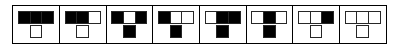
\includegraphics[width=.7\textwidth]{fig_ruleIcon60.png}
	  \caption{Tabela de transições da regra 60 do espaço elementar.}
	  \label{fig:table60}
	\end{figure}

	\begin{figure}[h!]
	  \centering
	  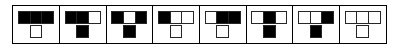
\includegraphics[width=.7\textwidth]{fig_ruleIcon102.png}
	  \caption{Tabela de transições da regra 102 do espaço elementar, obtida através da transformação de reflexão aplicada na tabela de transições da regra 60.}
	  \label{fig:table102}
	\end{figure}

Ao se aplicar a transformação por conjugação na regra 60 obtemos a regra 195 do espaço elementar, conforme ilustrado na Figura \ref{fig:table195}. E por fim, ao se aplicar a transformação por composição de reflexão e conjugação na regra 60 obtemos a regra 153 do espaço elementar, conforme ilustrado na Figura \ref{fig:table153}.

	\begin{figure}[h!]
	  \centering
	  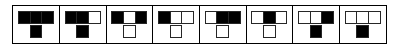
\includegraphics[width=.7\textwidth]{fig_ruleIcon195.png}
	  \caption{Tabela de transições da regra 195 do espaço elementar, obtida através da transformação de conjugação aplicada na tabela de transições da regra 60.}
	  \label{fig:table195}
	\end{figure}

	\begin{figure}[h!]
	  \centering
	  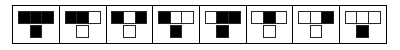
\includegraphics[width=.7\textwidth]{fig_ruleIcon153.png}
	  \caption{Tabela de transições da regra 153 do espaço elementar, obtida através da transformação de composição aplicada na tabela de transições da regra 60.}
	  \label{fig:table153}
	\end{figure}

Tanto a regra 60, como as regras 102, 153 e 195 pertencem a mesma classe de equivalência dinâmica. Uma forma interessante de entender o porquê é analisando a evolução espaço-temporal dessas regras, ilustrada pela Figura \ref{fig:dynamicEquivalecy}.

	\begin{figure}[h!]
	  \centering
	  \def\svgscale{0.63}
	  \import{./img/}{fig_ruleEquivalence60.pdf_tex}
	  \caption{Evolução espaço-temporal das regras pertencente à mesma classe dinâmica da regra 60.}
	  \label{fig:dynamicEquivalecy}
	\end{figure}

Tendo em vista as tabelas de transições obtidas por meio das transformações, é possível saber quão simétrica é uma regra, ou em outras palavras, qual a simetria interna de uma regra em relação a uma determinada transformação. A simetria interna pode ser representada pelo número de vizinhanças que permanecem iguais após aplicada uma determinada transformação. Exemplificando, a regra 60 dos ACs elementares tem um valor de simetria interna por reflexão igual a 4, pois compartilha as transições de estado $((1,1,1),0)$, $((1,0,1),1)$, $((0,1,0),1)$ e $ ((0,0,0),0)$ com a regra resultante de sua transformação por reflexão, a regra 102. Vale notar que as vizinhanças compartilhadas são todas as vizinhanças invariantes do espaço elementar, logo pode-se dizer que a regra 60 tem a menor simetria interna possível para o espaço elementar.

Um resultado bem diferente pode ser visto ao se repetir esse mesmo processo para a regra 204, que tem o valor 8 de simetria interna para transformação por reflexão. Esse valor é máximo possível para o espaço elementar e evidencia que ao se aplicar a transformação por reflexão na regra 204 será obtida a mesma regra como resultado. Uma regra contiver máxima simetria para uma transformação é uma regra invariante.

Vale frisar que apenas transformações por reflexão apresentam vizinhanças invariantes. No caso das reflexões por conjugação e por composição isso não ocorre.

Já há implementado no CATemplates um algoritmo gerador de templates que representam regras do espaço binário com um determinado valor de simetria para uma transformação.

O algoritmo recebe como parâmetro um raio $r$, definindo assim a família de ACs que será representada, o valor de simetria interna desejado, e uma das transformações de simetria.

Para melhor representar o funcionamento do algoritmo, considere que foi passado como parâmetro um raio $r = 1$, a transformação de reflexão e a simetria interna desejada igual a 8. O primeiro passo do algoritmo será gerar todas as vizinhanças do espaço, que no nosso exemplo pode ser representado pela conjunto descrito pela Eq. \eqref{eq:neighborSetACE}
\begin{equation}
\{(1,1,1),(1,1,0),
(1,0,1),(1,0,0),
(0,1,1),(0,1,0),
(0,0,1),(0,0,0)\}
\label{eq:neighborSetACE}
\end{equation}

Após isso, a transformação escolhida, no caso reflexão, é aplicada a cada uma das vizinhanças, gerando assim o conjunto representado pela Eq. \eqref{eq:neighborSetTransformadoACE}.  
\begin{equation}
\begin{split}
\{
((1,1,1),(1,1,1)),
((1,1,0),(0,1,1)),
((1,0,1),(1,0,1)),
((1,0,0),(0,0,1)),\\
((0,1,1),(1,1,0)),
((0,1,0),(0,1,0)),
((0,0,1),(1,0,0)),
((0,0,0),(0,0,0))\}
\label{eq:neighborSetTransformadoACE}
\end{split}
\end{equation}

Então, dos pares de vizinhanças encontrados, salva-se em uma variável o número de vizinhanças invariantes à transformação escolhida e remove-se os pares de vizinhanças idênticos. Após essa operação o conjunto resultante estará de acordo com a Eq. \eqref{eq:neighborSetTransformadoInACE}.
\begin{equation}
\{(((1,1,0),(0,1,1)),
((1,0,0),(0,0,1)),
((0,1,1),(1,1,0)),
((0,0,1),(1,0,0))\}
\label{eq:neighborSetTransformadoInACE}
\end{equation}

Nesse momento, caso o valor de simetria interna passado como parâmetro seja menor que as vizinhanças invariantes, o algoritmo retorna como resultado um conjunto vazio, tendo em vista que o valor mínimo de simetria interna é igual ao total de vizinhanças invariantes. Caso contrário o algoritmo agora removerá todas as repetições de pares de vizinhanças, considerando que pares de vizinhanças em ordem diferentes repetições. A Eq. \eqref{eq:internalSimetryP4} representa como ficara o conjunto após as remoções.
\begin{equation}
\{(((1,1,0),(0,1,1)), ((1,0,0),(0,0,1))\}
\label{eq:internalSimetryP4}
\end{equation}

Cada vizinhança é então substituída pela variável de template correspondente a sua posição, gerando assim um conjunto que representa as equivalências entre variáveis de um template. Esse conjunto de equivalências podem ser melhor visualizados pela Eq. \eqref{eq:internalSimetryP5} e pelo sistema de equação equivalente representado pela Eq. \eqref{eq:internalSimetryP6}.
\begin{equation}
\{(x_6,x_3), (x_4,x_1)\}
\label{eq:internalSimetryP5}
\end{equation}

\begin{equation}
\left\{\begin{matrix}
x_4 & = & x_1\\ 
x_6 & = & x_3
\end{matrix}\right.
\label{eq:internalSimetryP6}
\end{equation}

Entretanto, apesar de igualar todas o sistema de equações ser útil para encontrar a máxima simetria interna de uma determinada transformação, para outros valores de simetria entre o mínimo e o máximo, é necessário que o sistema de equações apresentem algumas inequações, como pode ser visualizado na Eq. \eqref{eq:internalSimetryP7} e na Eq. \eqref{eq:internalSimetryP8}.
\begin{equation}
\left\{\begin{matrix}
x_4 & \neq & x_1\\ 
x_6 & = & x_3
\end{matrix}\right.
\label{eq:internalSimetryP7}
\end{equation}

\begin{equation}
\left\{\begin{matrix}
x_4 & = & x_1\\ 
x_6 & \neq & x_3
\end{matrix}\right.
\label{eq:internalSimetryP8}
\end{equation}

A relação de desigualdade é representada nos templates por meio de uma função que sempre dê um resultado diferente. No caso binário essa função é $1 - x_i$. Logo os sistemas representados pela Eq. \eqref{eq:internalSimetryP7} e pela Eq. \eqref{eq:internalSimetryP8} são respectivamente equivalentes a Eq. \eqref{eq:internalSimetryP9} e a Eq. \eqref{eq:internalSimetryP10}
\begin{equation}
\left\{\begin{matrix}
x_4 & = & 1 - x_1\\ 
x_6 & = & x_3
\end{matrix}\right.
\label{eq:internalSimetryP9}
\end{equation}

\begin{equation}
\left\{\begin{matrix}
x_4 & = & x_1\\ 
x_6 & = 1 - & x_3
\end{matrix}\right.
\label{eq:internalSimetryP10}
\end{equation}

Para montar essas equivalências, o algoritmo particiona o conjunto de equivalência em $(s-v)/2$ partes, sendo que $s$ é o número de simetria interna passado como argumento e $v$ é o número de vizinhanças invariantes à transformação determinada. Após o particionamento, o algoritmo une as partições com os complementos do conjunto, adicionando assim as desigualdades nos pares do complemento. Para os exemplos dados, o conjunto resultante é representado pela Eq. \eqref{eq:internalSimetryP11}.
\begin{equation}
C_{reflex6}=\{((x_4,x_1),(x_6,1-x_3)),((x_4,1-x_1),(x_6,x_3))\}
\label{eq:internalSimetryP11}
\end{equation}

O conjunto $C_{reflex6}$ representa as equivalências entre variáveis, que quando aplicadas ao template base, originam os templates que representam as regras com simetria interna 6. Ao realizar essas substituições obtemos o conjunto de templates representado pela Eq. \eqref{eq:internalSimetryP12}.

\begin{equation}
\{(x_7,1-x_3,x_5,x_1,x_3,x_2,x_1,x_0),(x_7,x_3,x_5,1-x_1,x_3,x_2,x_1,x_0)\}
\label{eq:internalSimetryP12}
\end{equation}
Esse conjunto de templates representam todas as regras com valor de simetria por reflexão igual a 6 do espaço elementar.

Esse algoritmo teve sua primeira implementação apresentada por De Oliveira e Verardo (\citeyear{deOliveira2014}; \citeyear{deOliveira2014b}). Posteriormente uma nova versão foi apresentada em \cite{Verardo2014}.

\subsection{Totalidade e Semi-totalidade}
Os ACs totalísticos são autômatos celulares cujo valor de uma célula depende apenas da soma dos valores dos seus vizinhos no passo de tempo anterior \cite{wolfram1983statistical}.

De forma análoga é possível dizer que as transições dependem da média das células que compõem  a vizinhança ao invés da soma. A Figura \ref{fig:totalistcRule} ilustra a tabela de transição do AC totalístico 777 com $k = 3$ e $r = 1$. 

	\begin{figure}[h!]
	  \centering
	  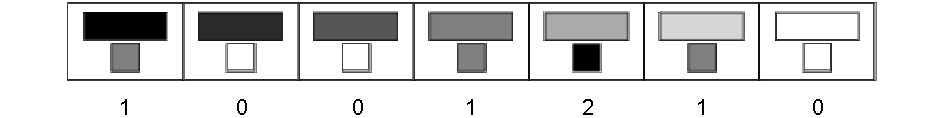
\includegraphics[width=1\textwidth]{fig_totalistcRule777.pdf}
	  \caption{Tabela de transição do AC totalístico 777. As transições dependem da média dos estados das células da vizinhança. Cada média possível é representada por tons de cinza entre o branco (estado 0) e o preto (estado 2).}
	  \label{fig:totalistcRule}
	\end{figure}

Já os ACs semi-totalísticos (\textit{outer-totalistic CA}) são generalizações de ACs totalísticos \cite{weisstein2015outerTotalistic}. Um AC pode ser considerado semi-totalístico caso suas transições sejam definidas pela soma (ou média) das células da vizinhança sem levar em consideração a célula central.

%talvez trocar citação de Gardner.
O Jogo da Vida \cite{GardnerM1970} é o exemplo mais conhecido de autômatos celulares semi-totalísticos, tendo em vista que as células centrais no Jogo da Vida são definidas em termos de ``viva'' (estado 1) ou ``morta'' (estado 0).

Os ACs semi-totalísticos podem ser interpretados como ACs clássicos que apresentam a propriedade de \textit{semi-totalidade}. A propriedade de semi-totalidade determina que as transições que apresentem a mesma soma dos estados vizinhos externos e que tenham a mesma célula central devem apresentar o mesmo resultado. Da mesma forma os ACs totalísticos também tem sua propriedade correspondente nos ACs clássicos: a \textit{totalidade}. A totalidade determina que todas as transições que apresentem a mesma soma dos estados das vizinhanças devem levar a um mesmo resultado.

A partir das definições de como devem ser as transições de estados dos ACs totalísticos e dos ACs semi-totalísticos foi possível representá-los por meio de templates. A biblioteca \textit{CATemplates} já apresenta os algoritmos que geram essas propriedades e seu funcionamento é bem simples. 

O algoritmo que gera regras totalísticas recebe como argumento os valores de $r$ e $k$, definindo assim uma família de ACs. Em seguida enumera as vizinhanças do espaço e calcula a soma dos estados de cada uma delas. O resultado da soma é o que define quais transições devem ser iguais para que o template represente apenas regras totalísticas.

Para determinar qual será a variável associada, dada uma vizinhança qualquer, o algoritmo verifica se a vizinhança foi a única até então que obteve um determinado valor de soma. Em caso positivo o algoritmo criará e associará uma variável $x_i$ para esta transição, sendo $i$ o valor decimal da vizinhança. Caso contrário, a transição será associada uma variável $x_i$ em que $i$ é o valor decimal da primeira e menor vizinhança encontrada com o mesmo valor de soma das vizinhanças.

A Eq. \eqref{eq:templateTotalisticECA} representa o template para o espaço elementar gerado pelo processo descrito acima. Esse template, quando expandido, gera $k^m = 2^4 = 16$ regras.
\begin{equation}
\begin{split}
(x_7,x_3,x_3,x_1,x_3,x_1,x_1,x_0)
\label{eq:templateTotalisticECA}
\end{split}
\end{equation}

Já para a família de ACs de $k=3$ e $r=1$, o algoritmo gera o template demonstrado pela Eq. \eqref{eq:templateTotalistic31}, sendo que esse template representa as $k^m = 3^7 = 2.187$ regras totalísticas do espaço.
\begin{equation}
\begin{split}
(x_{26},x_{17},x_8,x_{17},x_8,x_5,x_8,x_5,x_2,x_{17},x_8,x_5,x_8,\\
x_5,x_2,x_5,x_2,x_1,x_8,x_5,x_2,x_5,x_2,x_1,x_2,x_1,x_0)
\label{eq:templateTotalistic31}
\end{split}
\end{equation}

Para as regras semi-totalísticas, o algoritmo segue o mesmo processo básico, porém com uma pequena modificação: as vizinhanças são somadas, mas a célula central é desconsiderada na soma e posteriormente concatenada ao final do resultado. Neste processo as vizinhanças que contenham o mesmo estado na célula central e a mesma soma de valores dos estados das células externas, como por exemplo $(2,1,0)$ e $(1,1,1)$, geram a mesma cadeias de caracteres ao final. A partir desse ponto o algoritmo segue a mesmo processo aplicado as regras totalísticas: para determinar qual será a variável associada a uma vizinhança o algoritmo verifica se a vizinhança foi a única até então que obteve um determinado valor. Em caso positivo o algoritmo criará e associará uma variável $x_i$ para esta transição, sendo $i$ o valor decimal da vizinhança. Caso contrário, a transição será associada uma variável $x_i$ em que $i$ é o valor decimal da primeira e menor vizinhança encontrada com o mesmo valor de soma das vizinhanças.

Aplicando esse algoritmo gerador de templates de regras semi-totalísticas como os argumentos $k=2$ e $r=1$ é obtido o template representado pela Eq. \eqref{eq:templateSemiTotalisticECA}.
\begin{equation}
\begin{split}
(x_7,x_3,x_5,x_1,x_3,x_2,x_1,x_0)
\label{eq:templateSemiTotalisticECA}
\end{split}
\end{equation}

O template representado pela Eq. \eqref{eq:templateSemiTotalisticECA} quando expandido gera as $k^m = 2^6 = 64$ regras semi-totalísticas do espaço elementar.

Para a família de ACs com $k=3$ e $r=1$, o algoritmo gera o template representado pela Eq. \eqref{eq:templateSemiTotalistic31}, que quando expandida gera as $k^m = 3^{15} = 14.348.907$ regras semi-totalísticas do espaço.
\begin{equation}
\begin{split}
(x_{26},x_{17},x_8,x_{23},x_{14},x_5,x_{20},x_{11},x_2,x_{17},x_8,x_7,x_{14},\\
x_5,x_4,x_{11},x_2,x_1,x_8,x_7,x_6,x_5,x_4,x_3,x_2,x_1,x_0)
\label{eq:templateSemiTotalistic31}
\end{split}
\end{equation}